% lecture13.tex — Winding Number and Borsuk-Ulam Theorem

\section{Winding Numbers}

\begin{definition}{Winding Number}{winding-number}
    Let $M$ be a compact, connected $(n-1)$-manifold and $f \colon M \to \R^n$ a smooth map. If $z \in \R^n$ is not in the image of $f$, consider the map
    \[
        u \colon M \to S^{n-1}, \qquad x \mapsto \frac{f(x) - z}{|f(x) - z|}.
    \]
    Define the \emph{mod 2 winding number} of $f$ around $z$ to be the mod 2 degree of $u$, i.e.
    \[
        \operatorname{wind}_{\Z/2}(f, z) := \deg_{\Z/2}(u).
    \]
\end{definition}

\begin{center}
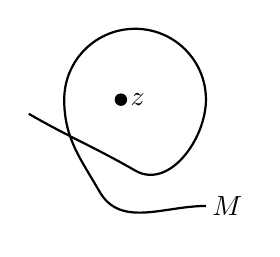
\begin{tikzpicture}[scale=0.9]
    % Curve M
    \draw[thick] (0,0.8) to[out=-30,in=150] (1.5,0) to[out=-30,in=270] (2.5,1) to[out=90,in=0] (1.5,2) to[out=180,in=90] (0.5,1) to[out=270,in=120] (1,-0.3) to[out=300,in=180] (2.5,-0.5);
    \node at (2.8,-0.5) {$M$};
    % Point z
    \fill (1.3,1) circle (2.5pt) node[right] {$z$};
\end{tikzpicture}
\end{center}

\begin{theorem}{Winding Number Formula}{winding-formula}
    Suppose $M = \partial D$ for some compact $n$-manifold $D$ with boundary, and let $F \colon D \to \R^n$ be a map extending $f$. If $z \in \R^n$ is a regular value of $F$ that's not in the image of $f$, then
    \[
        \operatorname{wind}_{\Z/2}(f, z) = \# F^{-1}(z) \mod 2.
    \]
\end{theorem}

\begin{proof}
    If $z$ is not in the image of $F$, then $u$ extends to $D$, so $\deg_{\Z/2}(u) = 0$ in that case.

    If $F^{-1}(z) = \{y_1, \ldots, y_\ell\}$, then $F$ is a local diffeomorphism at each $y_i$, $1 \leq i \leq \ell$, so we can choose a small ball $B_i$ around $y_i$ such that $u_i \colon \partial B_i \to S^{n-1}$ is bijective (and hence $\operatorname{wind}_{\Z/2}(f_i, z) = 1$), where $f_i := F|_{\partial B_i}$. We may assume that the balls are disjoint from each other and from $M = \partial D$.

    But our previous observation (applied to $D' = D - \bigcup_{i=1}^{\ell} \operatorname{Int}(B_i)$) implies
    \[
        \operatorname{wind}_{\Z/2}(f, z) = \operatorname{wind}_{\Z/2}(f_1, z) + \cdots + \operatorname{wind}_{\Z/2}(f_\ell, z) \mod 2 = \# F^{-1}(z) \mod 2.
    \]
    \begin{center}
    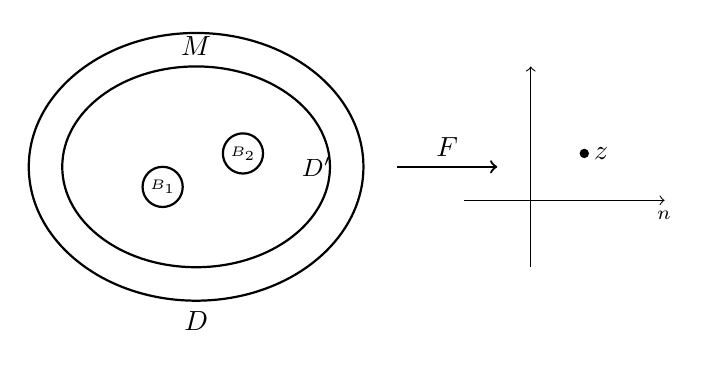
\begin{tikzpicture}[scale=0.85]
        % D' (D with balls removed)
        \draw[thick] (0,0) ellipse (2 and 1.5);
        \node at (0,1.8) {$M$};
        \draw[thick] (0,0) ellipse (2.5 and 2);
        \node at (0,-2.3) {$D$};
        % Small balls removed
        \draw[thick,fill=white] (-0.5,-0.3) circle (0.3);
        \node at (-0.5,-0.3) {\tiny $B_1$};
        \draw[thick,fill=white] (0.7,0.2) circle (0.3);
        \node at (0.7,0.2) {\tiny $B_2$};
        \node at (1.8,0) {\small $D'$};
        % Arrow
        \draw[->,thick] (3,0) -- (4.5,0) node[midway,above] {$F$};
        % R^n
        \draw[->] (5,-1.5) -- (5,1.5);
        \draw[->] (4,-0.5) -- (7,-0.5);
        \node at (7,-0.8) {$\R^n$};
        \fill (5.8,0.2) circle (2pt) node[right] {$z$};
    \end{tikzpicture}
    \end{center}
\end{proof}

\subsection{Jordan--Brouwer Separation Theorem}

When $M$ is a compact, connected hypersurface in $\R^n$ (i.e.\ codimension 1 submanifold), we can use the winding numbers to prove:

\begin{theorem}{Jordan--Brouwer Separation Theorem}{jordan-brouwer}
    The complement of a compact, connected hypersurface $M$ in $\R^n$ consists of two connected open sets, the ``outside'' $D_0$ and the ``inside'' $D_1$. Moreover, $\bar{D}_1$ is a compact $n$-manifold with boundary $\partial \bar{D}_1 = M$.
\end{theorem}

\begin{proof}[Proof sketch]
    Let $D_a := \{z \in \R^n \setminus M \mid \operatorname{wind}_{\Z/2}(M, z) = a\}$ for each $a \in \Z/2$, so that $\R^n \setminus M = D_0 \sqcup D_1$. Since $\operatorname{wind}_{\Z/2}(M, z)$ is locally constant, they are both open.

    For each $x \in M$, if $B$ is a small open ball around $x$ in $\R^n$, then $B \setminus M = B_0 \sqcup B_1$, where $B_0, B_1$ are two connected half balls, and $B_a = D_a \cap B$.

    \begin{center}
    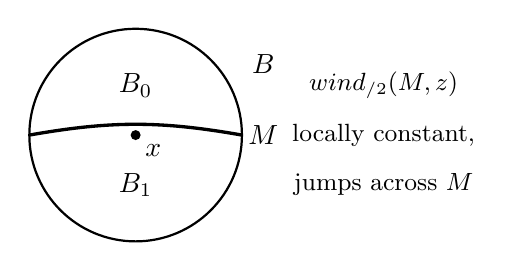
\begin{tikzpicture}[scale=0.9]
        % Ball B
        \draw[thick] (0,0) circle (1.5);
        \node at (1.8,1) {$B$};
        % M cutting through
        \draw[very thick] (-1.5,0) to[out=10,in=170] (1.5,0);
        \node at (1.8,0) {$M$};
        % Labels
        \node at (0,0.7) {$B_0$};
        \node at (0,-0.7) {$B_1$};
        \fill (0,0) circle (2pt) node[below right] {$x$};
        % Winding number annotation
        \node at (3.5,0.7) {\small $\operatorname{wind}_{\Z/2}(M,z)$};
        \node at (3.5,0) {\small locally constant,};
        \node at (3.5,-0.7) {\small jumps across $M$};
    \end{tikzpicture}
    \end{center}

    Connectivity of $M$ implies $D_a$ is connected, and compactness of $M$ implies $\bar{D}_1$ is compact.
\end{proof}

\section{Borsuk--Ulam Theorem}

\begin{theorem}{Borsuk--Ulam Theorem}{borsuk-ulam}
    Let $f \colon S^n \to \R^{n+1} \setminus \{0\}$ be a smooth map such that $f(-x) = -f(x)$ for all $x \in S^n$. Then $\operatorname{wind}_{\Z/2}(f, 0) = 1$.
\end{theorem}

\begin{proof}
    Let's proceed by induction on $n$.

    For $n = 1$, if $f \colon S^1 \to S^1$ is an antipodal map, then its lift $\tilde{f} \colon \R \to \R$ must satisfy $\tilde{f}(\theta + \pi) = \tilde{f}(\theta) + k\pi$ for some odd $k$, and $\deg_{\Z/2} f = k = 1 \pmod{2}$.

    Now assume the theorem for $n - 1$, and let $f \colon S^n \to \R^{n+1} \setminus \{0\}$ be antipodal. The idea is to compute $\operatorname{wind}_{\Z/2}(f, 0)$ by $I_2(f, R)$ for some ray $R$ from $0$.

    Let $g = f|_{S^{n-1}}$ (the equator $S^n \cap \{x_{n+1} = 0\}$) and use Sard to choose a unit vector $v$ that is a regular value for both $\frac{g}{|g|} \colon S^{n-1} \to S^n$ and $\frac{f}{|f|} \colon S^n \to S^n$.

    Let $\ell = \R \cdot v$ be the corresponding line. Then $f \pitchfork \ell$, and $g$ never intersects $\ell$.

    Now,
    \[
        \operatorname{wind}_{\Z/2}(f, 0) = \deg_{\Z/2}\!\left(\frac{f}{|f|}\right) = \#\left(\frac{f}{|f|}\right)^{-1}(v) \mod 2 = \frac{1}{2} \# f^{-1}(\ell) = \# f_+^{-1}(\ell) \mod 2,
    \]
    where $f_+ = f|_{S^n_+}$ is the restriction to the upper hemisphere.

    \begin{center}
    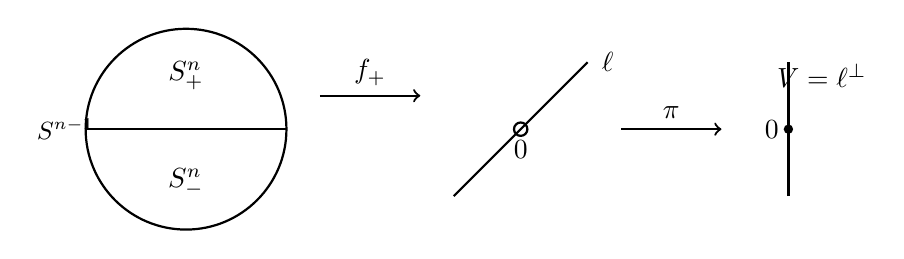
\begin{tikzpicture}[scale=0.85]
        % S^n (circle representation)
        \draw[thick] (0,0) circle (1.5);
        \draw[thick] (-1.5,0) -- (1.5,0);
        \node at (0,0.8) {$S^n_+$};
        \node at (0,-0.8) {$S^n_-$};
        \node at (-1.8,0) {\small $S^{n-1}$};
        % Arrow f_+
        \draw[->,thick] (2,0.5) -- (3.5,0.5) node[midway,above] {$f_+$};
        % Target with line l
        \draw[thick] (5,0) circle (0.1);
        \node at (5,-0.3) {$0$};
        \draw[thick] (4,-1) -- (6,1);
        \node at (6.3,1) {$\ell$};
        % Arrow pi
        \draw[->,thick] (6.5,0) -- (8,0) node[midway,above] {$\pi$};
        % V = l^perp
        \draw[thick] (9,-1) -- (9,1);
        \node at (9.5,0.8) {$V = \ell^\perp$};
        \fill (9,0) circle (2pt) node[left] {$0$};
    \end{tikzpicture}
    \end{center}

    By induction hypothesis,
    \[
        \operatorname{wind}_{\Z/2}(f, 0) = \# f_+^{-1}(\ell) = \#(\pi \circ f_+)^{-1}(0) = \operatorname{wind}_{\Z/2}\!\left(\pi \circ g, 0\right) = 1 \mod 2.
    \]
\end{proof}

\begin{corollary}{}{borsuk-ulam-cor1}
    If $f \colon S^n \to \R^{n+1} \setminus \{0\}$ is antipodal, then $f$ intersects every line through $0$ at least once.
\end{corollary}

\begin{corollary}{}{borsuk-ulam-cor2}
    For any $n$ smooth functions $g_1, \ldots, g_n$ on $S^n$, such that $g_i(p) = g_i(-p)$ for all $i = 1, \ldots, n$, there exists a point $p \in S^n$ at which all $g_i$ vanish simultaneously.
\end{corollary}

\begin{proof}
    If not, apply the corollary to the map $f(x) = (g_1(x) - g_1(-x), \ldots, g_n(x) - g_n(-x), 0)$ and take the $x_{n+1}$ axis for $\ell$.
\end{proof}
